\documentclass[letterpaper, 11pt]{extarticle}
% \usepackage{fontspec}

% ==================================================

% document parameters
% \usepackage[spanish, mexico, es-lcroman]{babel}
\usepackage[utf8]{inputenc}
\usepackage[english, russian]{babel}
\usepackage[margin = 1in]{geometry}
\usepackage{setspace}
% \usepackage[paper=a4paper, left=15mm, right=15mm, top=20mm, bottom=20mm]{geometry}

% ==================================================

% Packages for math
\usepackage{mathrsfs}
\usepackage{amsfonts}
\usepackage{amsmath}
\usepackage{amsthm}
\usepackage{amssymb}
\usepackage{physics}
\usepackage{dsfont}
\usepackage{esint}
\usepackage{mathtools}

% ==================================================

% Packages for writing
\usepackage{enumerate}
\usepackage[shortlabels]{enumitem}
\usepackage{framed}
\usepackage{csquotes}

% ==================================================

% Miscellaneous packages
\usepackage{float}
\usepackage{tabularx}
\usepackage{xcolor}
\usepackage{multicol}
\usepackage{subcaption}
\usepackage{caption}
\usepackage{fancyhdr}
\usepackage{graphicx}
\captionsetup{format = hang, margin = 10pt, font = small, labelfont = bf}

% Citation
\usepackage[round, authoryear]{natbib}

% Hyperlinks setup
\usepackage{hyperref}
\definecolor{links}{rgb}{0.36,0.54,0.66}
\hypersetup{
   colorlinks = true,
    linkcolor = black,
     urlcolor = blue,
    citecolor = blue,
    filecolor = blue,
    pdfauthor = {Author},
     pdftitle = {Title},
   pdfsubject = {subject},
  pdfkeywords = {one, two},
  pdfproducer = {LaTeX},
   pdfcreator = {pdfLaTeX},
}


\pagestyle{empty}

\begin{document}

\begin{singlespace}
\setstretch{1}

\parbox{\textwidth}{
    \centering{
        МИНИСТЕРСТВО ОБРАЗОВАНИЯ И НАУКИ РОССИЙСКОЙ ФЕДЕРАЦИИ\\
        ГОСУДАРСТВЕННОЕ БЮДЖЕТНОЕ ОБРАЗОВАТЕЛЬНОЕ УЧРЕЖДЕНИЕ\\
        ВЫСШЕГО ПРОФЕССИОНАЛЬНОГО ОБРАЗОВАНИЯ
    }
}

\vspace{5em}

\parbox{\textwidth}{
    \centering{
        \guillemotleft Московский государственный технический\\
        университет имени Н.Э. Баумана\guillemotright\\
        (МГТУ им. Н.Э. Баумана)}
}

\vspace{5em}

\parbox{\textwidth}{
    \centering{
        ФАКУЛЬТЕТ ФУНДАМЕНТАЛЬНЫХ НАУК\\
        КАФЕДРА\\
        \guillemotleft ВЫЧИСЛИТЕЛЬНАЯ МАТЕМАТИКА И МАТЕМАТИЧЕСКАЯ ФИЗИКА\guillemotright
    }
}

\vspace{3em}

\parbox{\textwidth}{
    \centering{
        Направление: \textbf{Математика и компьютерные науки}
    }
}

\vspace{3em}

\parbox{\textwidth}{
    \centering{
        Дисциплина: Численные методы
    }
}

\vspace{3em}

\parbox{\textwidth}{
    \centering{
        Домашняя работа №1.2\\
        \guillemotleft Метод наименьших квадратов и модели регрессии\guillemotright\\
        Группа ФН11-52Б
    }
}

\vspace{3em}

\parbox{\textwidth}{
    \centering{
        Вариант №9
    }
}

\vspace{3em}

\parbox{\textwidth}{
    \raggedleft{
        Студент: Очкин Н.В.
    }
}

\vspace{3em}

\parbox{\textwidth}{
    \raggedleft{
        Преподаватель:  Кутыркин В.А.
    }
}

\vspace{3em}

\parbox{\textwidth}{
    \centering{
        Оценка:
    }
}

\vspace{7em}

\parbox{\textwidth}{
    \centering{
        Москва, 2024
    }
}

\end{singlespace}

\newpage

\doublespacing

\section*{\centering{Задание 2.1}}

Дана модель линейной регрессии:

\begin{equation}
	Y = x^0_* + z_1x^1_* + z_2x^2_* + z_3x^3_* + z_4x^4_* + z_5x^5_* + z_6x^6_* + \varepsilon
\end{equation}

Для оценки неизвестных вектора тренда 
$\prescript{>}{}{x_*} = \left[ x^0_*, x^1_*, \dots, x^k_* \right> \in \prescript{>}{}{\mathbb{E}^{k+1}}$
и параметра $\sigma$ от случайной составляющей $\varepsilon \sim \mathcal{N}(0, \sigma)$ модели линейной регрессии (1). 
проводился эксперимент, в котором получены $m = 20$ значений $y^1, \dots, y^m \in \mathbb{R}$
регрессора модели (1) для $m$ различных наборов 
$\prescript{<}{}{z^1} = \left< z^1_1, \dots,  z^1_6\right], \dots, \prescript{<}{}{z^m} = \left< z^m_1, \dots,  z^m_6\right] 
\in \in \prescript{<}{}{\mathbb{R}^{6}}$ шести факторов модели (1).

Требуется получить оценки вектора тренда
$\prescript{>}{}{x_*} = \left[ x^0_*, x^1_*, \dots, x^k_* \right> \in \prescript{>}{}{\mathbb{E}^{k+1}}$
и параметра $\sigma$ от случайной составляющей $\varepsilon \sim \mathcal{N}(0, \sigma)$ модели линейной регрессии (1). 
Если возможно, редуцировать модель регрессии (1) до приведённой модели. 
Результаты расчётов проиллюстрировать графически, сопроводив их необходимыми комментариями.

\vspace{-0.75\baselineskip}

\section*{\centering{ \large Решение}}

\vspace{-0.75\baselineskip}

\begin{equation*}
    \textrm{N} = 9, \alpha = -0.025
\end{equation*}

\renewcommand{\arraystretch}{0.65}
\begin{center}
    \begin{tabular}{ | c | c | c | c | c | c | c | c | } 
      \hline
      $\textrm{z}^1$ & $\textrm{z}^2$ & $\textrm{z}^3$ & $\textrm{z}^4$ & $\textrm{z}^5$ & $\textrm{z}^6$ & $\textrm{y} + \alpha$ & $\textrm{y}$ \\
      \hline
      1.158574 & 1.194067 & 1.745872 & 1.566271 & 1.825556 & 1.942503 & 14.77 & 14.795 \\ 
      \hline 
      1.238868 & 1.913419 & 1.182653 & 1.044649 & 1.304209 & 1.924039 & 13.41 & 13.435 \\ 
      \hline 
      1.564043 & 1.561357 & 1.070589 & 1.778954 & 1.226447 & 1.824122 & 13.84 & 13.865 \\ 
      \hline 
      1.737266 & 1.798975 & 1.952239 & 1.752281 & 1.247871 & 1.54796 & 13.6 & 13.625 \\ 
      \hline 
      1.364544 & 1.03122 & 1.380596 & 1.688101 & 1.987396 & 1.058504 & 13.23 & 13.255 \\ 
      \hline 
      1.535295 & 1.742973 & 1.580401 & 1.063356 & 1.999237 & 1.425459 & 14.88 & 14.905 \\ 
      \hline 
      1.780725 & 1.306711 & 1.972594 & 1.68627 & 1.582629 & 1.767235 & 15.39 & 15.415 \\ 
      \hline 
      1.135044 & 1.139164 & 1.686178 & 1.220069 & 1.034577 & 1.019745 & 9.56 & 9.585 \\ 
      \hline 
      1.246498 & 1.114597 & 1.079653 & 1.333415 & 1.054445 & 1.156743 & 10.37 & 10.395 \\ 
      \hline 
      1.416456 & 1.349223 & 1.68038 & 1.003235 & 1.471908 & 1.095523 & 11.95 & 11.975 \\ 
      \hline 
      1.611866 & 1.972991 & 1.443953 & 1.014008 & 1.91699 & 1.182531 & 14.13 & 14.155 \\ 
      \hline 
      1.520585 & 1.427992 & 1.464156 & 1.011505 & 1.108341 & 1.981536 & 13.83 & 13.855 \\ 
      \hline 
      1.229896 & 1.304392 & 1.852107 & 1.705496 & 1.725639 & 1.21482 & 12.51 & 12.535 \\ 
      \hline 
      1.726829 & 1.866756 & 1.074984 & 1.09888 & 1.983154 & 1.256935 & 14.9 & 14.925 \\ 
      \hline 
      1.77279 & 1.363353 & 1.227454 & 1.076754 & 1.656758 & 1.675253 & 15.31 & 15.335 \\ 
      \hline 
      1.418256 & 1.072481 & 1.123447 & 1.438917 & 1.059481 & 1.080325 & 10.67 & 10.695 \\ 
      \hline 
      1.119724 & 1.947356 & 1.372631 & 1.635578 & 1.94058 & 1.112827 & 12.52 & 12.545 \\ 
      \hline 
      1.728446 & 1.802332 & 1.365001 & 1.184759 & 1.119633 & 1.880032 & 14.18 & 14.205 \\ 
      \hline 
      1.161107 & 1.359294 & 1.956206 & 1.143406 & 1.49144 & 1.688437 & 13.02 & 13.045 \\ 
      \hline 
      1.963561 & 1.271859 & 1.250008 & 1.19367 & 1.466262 & 1.624409 & 15.16 & 15.185 \\ 
      \hline 
    \end{tabular}
\end{center}

Разобъем данные на \textrm{\textbf{Z}} - матрица регрессоров (с добавлением свободного члена) и \textrm{\textbf{Y}} - вектор наблюдений:

\renewcommand{\arraystretch}{0.65}
\begin{center}
    \textrm{\textbf{Z}} = \begin{tabular}{ | c | c | c | c | c | c | c | } 
    \hline
    $\textrm{z}^0$ & $\textrm{z}^1$ & $\textrm{z}^2$ & $\textrm{z}^3$ & $\textrm{z}^4$ & $\textrm{z}^5$ & $\textrm{z}^6$ \\
    \hline
    1.0 & 1.158574 & 1.194067 & 1.745872 & 1.566271 & 1.825556 & 1.942503 \\ 
    \hline 
    1.0 & 1.238868 & 1.913419 & 1.182653 & 1.044649 & 1.304209 & 1.924039 \\ 
    \hline 
    1.0 & 1.564043 & 1.561357 & 1.070589 & 1.778954 & 1.226447 & 1.824122 \\ 
    \hline 
    1.0 & 1.737266 & 1.798975 & 1.952239 & 1.752281 & 1.247871 & 1.54796 \\
    \hline 
    1.0 & 1.364544 & 1.03122 & 1.380596 & 1.688101 & 1.987396 & 1.058504 \\ 
    \hline 
    1.0 & 1.535295 & 1.742973 & 1.580401 & 1.063356 & 1.999237 & 1.425459 \\ 
    \hline 
    1.0 & 1.780725 & 1.306711 & 1.972594 & 1.68627 & 1.582629 & 1.767235 \\ 
    \hline 
    1.0 & 1.135044 & 1.139164 & 1.686178 & 1.220069 & 1.034577 & 1.019745 \\  
    \hline 
    1.0 & 1.246498 & 1.114597 & 1.079653 & 1.333415 & 1.054445 & 1.156743 \\ 
    \hline 
    1.0 & 1.416456 & 1.349223 & 1.68038 & 1.003235 & 1.471908 & 1.095523 \\ 
    \hline 
    1.0 & 1.611866 & 1.972991 & 1.443953 & 1.014008 & 1.91699 & 1.182531 \\ 
    \hline 
    1.0 & 1.520585 & 1.427992 & 1.464156 & 1.011505 & 1.108341 & 1.981536 \\ 
    \hline 
    1.0 & 1.229896 & 1.304392 & 1.852107 & 1.705496 & 1.725639 & 1.21482 \\ 
    \hline 
    1.0 & 1.726829 & 1.866756 & 1.074984 & 1.09888 & 1.983154 & 1.256935 \\
    \hline 
    1.0 & 1.77279 & 1.363353 & 1.227454 & 1.076754 & 1.656758 & 1.675253 \\ 
    \hline 
    1.0 & 1.418256 & 1.072481 & 1.123447 & 1.438917 & 1.059481 & 1.080325 \\ 
    \hline 
    1.0 & 1.119724 & 1.947356 & 1.372631 & 1.635578 & 1.94058 & 1.112827 \\ 
    \hline 
    1.0 & 1.728446 & 1.802332 & 1.365001 & 1.184759 & 1.119633 & 1.880032 \\ 
    \hline 
    1.0 & 1.161107 & 1.359294 & 1.956206 & 1.143406 & 1.49144 & 1.688437 \\ 
    \hline 
    1.0 & 1.963561 & 1.271859 & 1.250008 & 1.19367 & 1.466262 & 1.624409 \\ 
    \hline 
    \end{tabular}
    \quad
    \textrm{\textbf{Y}} = \begin{tabular}{ | c | } 
        \hline
        $\textrm{y}$ \\
        \hline
        14.795 \\
        \hline
        13.435 \\
        \hline
        13.865 \\
        \hline
        13.625 \\ 
        \hline
        13.255 \\
        \hline
        14.905 \\
        \hline
        15.415 \\
        \hline
        9.585 \\ 
        \hline
        10.395 \\
        \hline
        11.975 \\
        \hline
        14.155 \\
        \hline
        13.855 \\
        \hline
        12.535 \\
        \hline
        14.925 \\ 
        \hline
        15.335 \\
        \hline
        10.695 \\
        \hline
        12.545 \\
        \hline
        14.205 \\
        \hline
        13.045 \\
        \hline
        15.185 \\
        \hline 
    \end{tabular}
\end{center}

Найдем число наблюдений \textrm{n} и количество регрессоров \textrm{k}: \\

\vspace{-1\baselineskip}

\begin{center}
    \textrm{n} = 20; \textrm{k} = 6
\end{center}

Для оценки параметров $\hat{\textrm{x}}$ применим метод наименьших квадратов (МНК):

\begin{equation*}
    \hat{\textrm{x}} = (\textrm{Z}^\textrm{T} \textrm{Z})^{-1}\textrm{Z}^\textrm{T} \textrm{Y} 
\end{equation*}

\vspace{-1\baselineskip}

\begin{equation*}
    \hat{\textrm{x}} = [0.01702005,   2.99863545,   0.00618907,  -0.00102846,   0.00046174,   2.99956383, 3.00008523] 
\end{equation*}

\newpage

Вычислим предсказания:

\begin{equation*}
    \hat{\textrm{y}} = [14.80102522, 13.42738099, 13.86772605, 13.62346337, 13.25145528, 
\end{equation*}

\vspace{-1.5\baselineskip}

\begin{equation*}
    14.90380052, 15.41265467,  9.58908442, 10.39441943, 11.97328504, 
\end{equation*}

\vspace{-1.5\baselineskip}

\begin{equation*}
    14.15944035, 13.85381575, 12.53271329, 14.92561512, 15.3360968,
\end{equation*}

\vspace{-1.5\baselineskip}

\begin{equation*}
    10.69504736, 12.54552937, 14.20896433, 13.04480987, 15.18367277] 
\end{equation*}

Найдем t-статистику и доверительный интервал:

\vspace{-1\baselineskip}

\begin{equation*}
    t_i = \frac{\hat{x_i}}{SE(\hat{x_i})} - \textrm{t-статистика}
\end{equation*}

\vspace{-1\baselineskip}

\begin{equation*}
    \hat{x_i} \pm t_{\alpha / 2} \cdot SE(\hat{x_i}) - \textrm{доверительный интервал}
\end{equation*}

где:

\vspace{-1\baselineskip}

\begin{align*}
    SE(\hat{x_i}) = \sqrt{\sigma^2 \cdot (Z^{\textrm{T}}Z)^{-1}_{ii}} - \textrm{стандартная ошибка} \\
    \sigma^2 = \frac{1}{n - k - 1} \sum_{i = 1}^{n} (y_i - \hat{y_i})^2 - \textrm{оценка дисперсии} 
\end{align*}

Для нахождения $t_{\alpha/2}$ воспользуемся модулем \textquote{\texttt{stats}} библиотеки \textquote{\texttt{scipy}}, которая динамически определит нужное критическое значение из таблицы Стьюдента в зависимости от заданных уровня значимости теста $\alpha$ (в данном случае 95\% для двустороннего интервала) и количества степеней свободы k (в данном случае n - k - 1 = 13)

\renewcommand{\arraystretch}{0.65}
\begin{center}
    \begin{tabular}{ | c | c | c | c | c | c | c | c | } 
      \hline
       & Y-пересечение & $\textrm{z}^1$ & $\textrm{z}^2$ & $\textrm{z}^3$ & $\textcolor{RED}{\textrm{z}^4}$ & $\textrm{z}^5$ & $\textrm{z}^6$ \\
      \hline
      Коэффициенты & 0.017 & 2.9986 & 0.0062 & -0.001 & \textcolor{RED}{0.0005} & 2.9996 & 3.0001 \\ 
      \hline 
      t-статистика & 1.7929 & 820.6219 & 2.0042 & -0.3436 & \textcolor{RED}{0.1451} & 1091.222 & 1062.342 \\ 
      \hline 
      Нижние 95\% & -0.0035 & 2.9907 & -0.0005 & -0.0075 & \textcolor{RED}{-0.0064} & 2.9936 & 2.994 \\ 
      \hline 
      Верхние 95\% & 0.0375 & 3.0065 & 0.0129 & 0.0054 & \textcolor{RED}{0.0073} & 3.0055 & 3.0062 \\ 
      \hline 
    \end{tabular}
\end{center}

\vspace{1\baselineskip}

Цветом выделен коэффициент $\textrm{z}^4$, т.к. модуль его t-статистики наименьший среди факторов, в доверительный интервал которых входит 0. Исключим $\textrm{z}^4$ и вычислим регрессию заново.

\renewcommand{\arraystretch}{0.65}
\begin{center}
    \begin{tabular}{ | c | c | c | c | c | c | c | } 
      \hline
       & Y-пересечение & $\textrm{z}^1$ & $\textrm{z}^2$ & $\textcolor{RED}{\textrm{z}^3}$ & $\textrm{z}^5$ & $\textrm{z}^6$ \\
      \hline
      Коэффициенты & 0.0176 & 2.9986 & 0.0061 & \textcolor{RED}{-0.001} & 2.9996 & 3.0001 \\ 
      \hline 
      t-статистика & 2.1664 & 852.139 & 2.0908 & \textcolor{RED}{-0.3347} & 1135.6755 & 1101.5763 \\ 
      \hline 
      Нижние 95\% & 0.0002 & 2.9911 & -0.0002 & \textcolor{RED}{-0.007} & 2.9939 & 2.9942 \\ 
      \hline 
      Верхние 95\% & 0.0351 & 3.0062 & 0.0124 & \textcolor{RED}{0.0051} & 3.0053 & 3.0059 \\ 
      \hline 
    \end{tabular}
\end{center}

\vspace{1\baselineskip}

Теперь исключим $\textrm{z}^3$.

\vspace{1\baselineskip}

\renewcommand{\arraystretch}{0.65}
\begin{center}
    \begin{tabular}{ | c | c | c | c | c | c | c | } 
      \hline
       & Y-пересечение & $\textrm{z}^1$ & $\textrm{z}^2$ & $\textrm{z}^5$ & $\textrm{z}^6$ \\
      \hline
      Коэффициенты & 0.0162 & 2.9988 & 0.0063 & 2.9994 & 2.9999 \\ 
      \hline 
      t-статистика & 2.4046 & 894.7026 & 2.2389 & 1195.9259 & 1158.7859 \\ 
      \hline 
      Нижние 95\% & 0.0018 & 2.9917 & 0.0003 & 2.9941 & 2.9944 \\ 
      \hline 
      Верхние 95\% & 0.0306 & 3.006 & 0.0122 & 3.0048 & 3.0054 \\ 
      \hline 
    \end{tabular}
\end{center}

\begin{center}
    \textbf{Оценка дисперсии $\sigma^2$ = 1e-05; $\sigma$ = 0.00357}
\end{center}

Построим график зависимости $\hat{\textrm{y}}$ от $\textrm{y}$:

\renewcommand{\arraystretch}{0.65}
\begin{center}
    \begin{tabular}{ | c | c | } 
    \hline
    $\hat{\textrm{y}}$ & $\textrm{y}$ \\
    \hline
    14.801 & 14.795 \\
    \hline
   13.4271 & 13.435 \\
    \hline
   13.8671 & 13.865 \\
    \hline
   13.6239 & 13.625 \\
    \hline
   13.2512 & 13.255 \\
    \hline
   14.904 & 14.905 \\
    \hline
   15.413 & 15.415 \\
    \hline
   9.5894 & 9.585 \\
    \hline
   10.3941 & 10.395 \\
    \hline
   11.9737 & 11.975 \\
    \hline
   14.1596 & 14.155 \\
    \hline
   13.8539 & 13.855 \\
    \hline
   12.5329 & 12.535 \\
    \hline
   14.9254 & 14.925 \\
    \hline
   15.336 & 15.335 \\
    \hline
   10.6947 & 10.695 \\
    \hline
   12.5453 & 12.545 \\
    \hline
   14.209 & 14.205 \\
    \hline
   13.0453 & 13.045 \\
    \hline
   15.1836 & 15.185 \\
    \hline 
    \end{tabular}
\end{center}

\begin{center}
    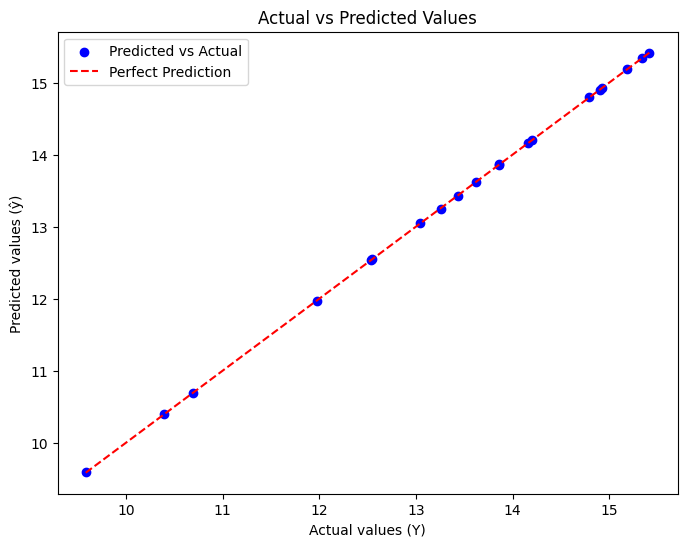
\includegraphics[width=15cm]{predictedVSy.png}
\end{center}

\textbf{Вывод:} предсказанный y ($\hat{y}$) и заданный y близки по значениями, так как их расхождение крайне мало.

\begin{equation*}
    \textrm{\textbf{Y}} = 0.0162 + 2.9988 \cdot \textrm{\textbf{z}}^1 + 0.0063 \cdot \textrm{\textbf{z}}^2 + 2.9994 \cdot \textrm{\textbf{z}}^5 + 2.9999 \cdot \textrm{\textbf{z}}^6
\end{equation*}

\newpage

\section*{\centering{Задание 2.2}}

Дана модель полиномиальной регрессии:

\begin{equation}
	Y = x^0_* + t \cdot x^1_* + t^2 \cdot x^2_* + t^3 \cdot x^3_* + \varepsilon
\end{equation}

Для оценки неизвестных вектора тренда 
$\prescript{>}{}{x_*} = \left[ x^0_*, x^1_*, x^3_*, x^4_* \right> \in \prescript{>}{}{\mathbb{E}^{4}}$
и параметра $\sigma$ от случайной составляющей $\varepsilon \sim \mathcal{N}(0, \sigma)$
модели полиномиальной регрессии (2) проводился эксперимент, в котором получены m = 20 значений
$y^1, \dots, y^m \in \mathbb{R}$  регрессора модели (2) для m попарно различных значений $t^1, \dots, t^m \in \mathbb{R}$ 
единственного фактора модели (2). Требуется получить оценки вектора тренда 
$\prescript{>}{}{x_*} = \left[ x^0_*, x^1_*, x^3_*, x^4_* \right> \in \prescript{>}{}{\mathbb{E}^{4}}$
и параметра $\sigma$ от случайной составляющей $\varepsilon \sim \mathcal{N}(0, \sigma)$ модели полиномиальной регрессии (2). 
Результаты расчётов проиллюстрировать графически, сопроводив их необходимыми комментариями.

\vspace{-0.75\baselineskip}

\section*{\centering{ \large Решение}}

\vspace{-0.75\baselineskip}

\begin{equation*}
    \textrm{N} = 9, \alpha = -0.025
\end{equation*}

\renewcommand{\arraystretch}{0.65}
\begin{center}
    \textrm{\textbf{T}} = \begin{tabular}{ | c | c | c | } 
    \hline
    $\textrm{t}$ & $\textrm{t}^2$ & $\textrm{t}^3$ \\
    \hline
    0.05 & 0.0025 & 0.0001 \\ 
    \hline 
   0.1 & 0.01 & 0.001 \\ 
    \hline 
   0.15 & 0.0225 & 0.0034 \\ 
    \hline 
   0.2 & 0.04 & 0.008 \\ 
    \hline 
   0.25 & 0.0625 & 0.0156 \\ 
    \hline 
   0.3 & 0.09 & 0.027 \\ 
    \hline 
   0.35 & 0.1225 & 0.0429 \\ 
    \hline 
   0.4 & 0.16 & 0.064 \\ 
    \hline 
   0.45 & 0.2025 & 0.0911 \\ 
    \hline 
   0.5 & 0.25 & 0.125 \\ 
    \hline 
   0.55 & 0.3025 & 0.1664 \\ 
    \hline 
   0.6 & 0.36 & 0.216 \\ 
    \hline 
   0.65 & 0.4225 & 0.2746 \\ 
    \hline 
   0.7 & 0.49 & 0.343 \\ 
    \hline 
   0.75 & 0.5625 & 0.4219 \\ 
    \hline 
   0.8 & 0.64 & 0.512 \\ 
    \hline 
   0.85 & 0.7225 & 0.6141 \\ 
    \hline 
   0.9 & 0.81 & 0.729 \\ 
    \hline 
   0.95 & 0.9025 & 0.8574 \\ 
    \hline 
   1.0 & 1.0 & 1.0 \\ 
    \hline 
    \end{tabular}
    \quad
    \textrm{\textbf{Y}} = \begin{tabular}{ | c | } 
        \hline
        $\textrm{y}$ \\
        \hline
        -4.725 \\
        \hline
        -4.535 \\
        \hline
        -4.315 \\
        \hline
        -4.145 \\
        \hline
        -3.955 \\
        \hline
        -3.795 \\
        \hline
        -3.625 \\
        \hline
        -3.455 \\
        \hline
        -3.285 \\
        \hline
        -3.105 \\
        \hline
        -2.905 \\
        \hline
        -2.695 \\
        \hline
        -2.465 \\
        \hline
        -2.215 \\
        \hline
        -1.925 \\
        \hline
        -1.615 \\
        \hline
        -1.265 \\
        \hline
        -0.885 \\
        \hline
        -0.455 \\
        \hline
        0.025 \\
        \hline
    \end{tabular}
\end{center}

Проведем вычисления, аналогичные заданию 2.1 в \textquote{\texttt{python}}\\
Результаты вычислений:

\renewcommand{\arraystretch}{0.65}
\begin{center}
    \begin{tabular}{ | c | c | c | c | c | } 
      \hline
       & Y-пересечение & $\textrm{t}$ & $\textrm{t}^2$ & $\textrm{t}^3$ \\
      \hline
      коэффициенты & -4.97013 & 4.94429 & -4.88082 & 4.92832 \\ 
       \hline 
      t-статистика & -752.32615 & 93.00244 & -42.01859 & 67.66452 \\ 
       \hline 
      нижние 95\% & -4.98413 & 4.83159 & -5.12706 & 4.77392 \\ 
       \hline 
      верхние 95\% & -4.95612 & 5.05699 & -4.63457 & 5.08273 \\ 
       \hline 
    \end{tabular}
\end{center}

\vspace{0.75\baselineskip}

\begin{center}
    \textbf{Оценка дисперсии $\sigma^2$ = 4e-05; $\sigma$ = 0.00605}
\end{center}

\vspace{0.75\baselineskip}

\renewcommand{\arraystretch}{0.65}
\begin{center}
    \begin{tabular}{ | c | c | c | } 
    \hline
    $\textrm{t}$ & $\hat{\textrm{y}}$ & $\textrm{y}$ \\
    \hline
    0.05 & -4.7345 & -4.725 \\ 
    \hline 
   0.1 & -4.51958 & -4.535 \\ 
    \hline 
   0.15 & -4.32167 & -4.315 \\ 
    \hline 
   0.2 & -4.13708 & -4.145 \\ 
    \hline 
   0.25 & -3.9621 & -3.955 \\ 
    \hline 
   0.3 & -3.79305 & -3.795 \\ 
    \hline 
   0.35 & -3.62622 & -3.625 \\ 
    \hline 
   0.4 & -3.45793 & -3.455 \\ 
    \hline 
   0.45 & -3.28447 & -3.285 \\ 
    \hline 
   0.5 & -3.10215 & -3.105 \\ 
    \hline 
   0.55 & -2.90727 & -2.905 \\ 
    \hline 
   0.6 & -2.69613 & -2.695 \\ 
    \hline 
   0.65 & -2.46504 & -2.465 \\ 
    \hline 
   0.7 & -2.21031 & -2.215 \\ 
    \hline 
   0.75 & -1.92823 & -1.925 \\ 
    \hline 
   0.8 & -1.61512 & -1.615 \\ 
    \hline 
   0.85 & -1.26727 & -1.265 \\ 
    \hline 
   0.9 & -0.88098 & -0.885 \\ 
    \hline 
   0.95 & -0.45257 & -0.455 \\ 
    \hline 
   1.0 & 0.02167 & 0.025 \\ 
    \hline 
    \end{tabular}
\end{center}

\begin{center}
    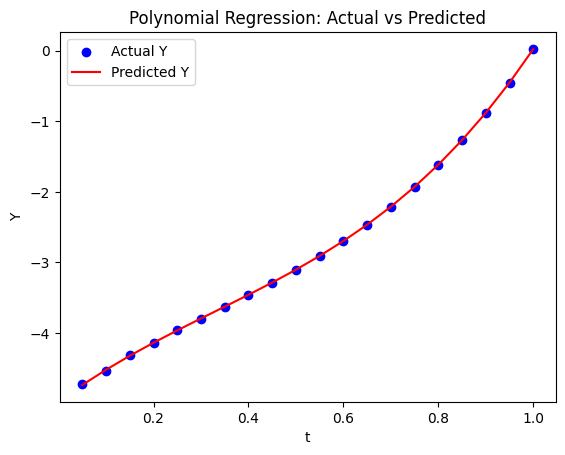
\includegraphics[width=15cm]{predictedVSy2.png}
\end{center}

\textbf{Вывод:} предсказанный y ($\hat{y}$) и заданный y близки по значениями, так как их расхождение крайне мало. Мы получили оценки вектора тренда
$\prescript{>}{}{x_*} = \left[ x^0_*, x^1_*, x^3_*, x^4_* \right> \in \prescript{>}{}{\mathbb{E}^{4}}$
и параметра $\sigma$ от случайной составляющей $\varepsilon \sim \mathcal{N}(0, \sigma)$ 
модели полиномиальной регрессии.

\begin{equation*}
    \textrm{\textbf{Y}} = -4.97012693 + 4.94428699 \cdot \textrm{\textbf{t}} - 4.88081748 \cdot \textrm{\textbf{t}}^2 + 4.92832484 \cdot \textrm{\textbf{t}}^3
\end{equation*}

\end{document}
